%---------------------------------------------------------------------------------------------------
\chapter{$f(Q)$ as Dark Energy}
\label{chap:STG-dark-energy}
%---------------------------------------------------------------------------------------------------

One of the major interests behind the study of modified gravity is to provide a theoretical explanation to dark energy.
Given that the model studied in the previous chapter is not able to explain the accelerated expansion of the universe without relying on a cosmological constant, in this chapter we will study an $f(Q)$ cosmological model where the modification to gravity accounts for its late time evolution. This model introduces a multiplicative term in the action that only modifies gravity in the low redshift regime. This extension of gravity does not add any extra degrees of freedom, given that it plays the role of a cosmological constant which, using the conservation equation, can be expressed as a function of both matter and radiation.

First, we will perform a dynamical system analysis\footnote{The main reference used for the theory behind the dynamical systems analysis was \cite{Strogatz}.} in order to narrow down the region in parameter space which provides viable cosmological models. Afterwards, we will use the \gls{SS} mock catalogs in order to distinguish this model from \gls{LCDM}. The usage of \gls{SNIa} will also be employed in order to assist in the model selection process, given that \gls{SS} alone are inconclusive.

This model was originally proposed in \cite{Anagnostopoulos2021}, where it was shown to be statistically equivalent to $\Lambda$CDM, for tests using \gls{SNIa}, redshift space distortions and cosmic chronometers. Additionally, it has been studied in \cite{Anagnostopoulos2022}, where it was shown to pass Big Bang nucleosynthesis constrains, showing that this modification to gravity is able to capture the accelerated expansion of the universe at late times, without modifying the early ages of the universe in a way that is compatible with observational data.


%---------------------------------------------------------------------------------------------------
\section{Dynamical System Analysis}
\label{sec:dynamical-system-analysis}
%---------------------------------------------------------------------------------------------------

As initially proposed in \cite{Anagnostopoulos2021}, we consider a specific form of the function  $f(Q)$ that replicates late time acceleration. We do this by introducing an extra term in the action that only impacts the low redshift regime, which caries an additional parameter $\lambda$, that plays the role of the cosmological constant. As for the energy matter content in the universe, we are dropping the assumption of the presence of a cosmological constant, and we consider a universe which is permeated solely by a perfect fluid composed of matter and radiation.

The action for this theory reads

\begin{equation}
    \label{eq:STG-dark-energy-model}
    f = Qe^{\lambda Q_0/Q} \,,
\end{equation}
where $Q_0$ is the non-metricity scalar, $Q=6H^2$, evaluated at the present day.

Rewriting the modified first Friedmann equation for a generic cosmological model of $f(Q)$ gravity, presented in \cref{eq:STG-friedmann-1}, by making use of the relative abundances, which were defined in \cref{eq:densities}, we obtain

\begin{equation}
    \label{eq:conservation}
    1 = \frac{1}{2} \frac{f}{Q f_Q}
    + \frac{1}{2 f_Q E^2}
    \left( \frac{\Omega_m}{a^3} + \frac{\Omega_r}{a^4}\right) \,.
\end{equation}
Computing the value of $f_Q$, and making use of the relationship between the non-metricity scalar and the Hubble function in \cref{eq:Q=6H2}, we obtain

\begin{equation}
    \label{eq:f_Q}
    f_Q = \left( 1 - \frac{\lambda}{E^2} \right) e^{\lambda/E^2} \,,
\end{equation}
which can be inserted back into \cref{eq:conservation} to give

\begin{equation}
    1 = \frac{e^{- \lambda / E^2}}{E^2} \left( \frac{\Omega_m}{a^3}
    + \frac{\Omega_r}{a^4} \right) + \frac{2\lambda}{E^2} \,.
\end{equation}
If we define the quantities

\begin{gather}
    x_1 \equiv \frac{\Omega_m}{E^2 e^{\lambda / E^2} a^3} \,, \hspace{1cm}
    x_2 \equiv \frac{\Omega_r}{E^2 e^{\lambda / E^2} a^4} \,, \hspace{1cm}
    x_3 \equiv \frac{2 \lambda}{E^2} \,,
\end{gather}
we can find a closed system of the form

\begin{equation}
    \label{eq:dynamical-system-conservation}
    x_1 + x_2 + x_3 = 1 \,.
\end{equation}

From the previous equation, we can see that the coordinate $x_1$ is related to the evolution of the matter density in the universe, whereas $x_2$ is related to the radiation density and $x_3$ to the contribution of our modification to gravity. Additionally, this equation shows that one of our coordinates in phase space is fully determined by the value of the other two. As such, without loss of generality, we choose to work only with $x_1$ and $x_2$.

In order to understand the evolution of the background dynamics of this universe, we introduce the number of e-folds, which is mathematically expressed as

\begin{equation}
    N \equiv \ln{a} \,,
\end{equation}
which we will now use as a proxy for time in our dynamical system. Computing the derivatives of the coordinates in phase space with respect to the number of e-folds, which from now one we will denote with a prime, reveals that

\begin{gather}
    x_1' = - x_1 \left(-(1+x_1+x_2)\frac{E'}{E} + 3\right) \,, \hspace{1cm}
    x_2' = - x_2 \left(-(1+x_1+x_2)\frac{E'}{E} + 4\right) \,,
\end{gather}
where the factor $E'/E$ can be expressed as a function of both $x_1$ and $x_2$ by


\begin{equation}
    \frac{E'}{E} \equiv \frac{3 x_1 + 4 x_2}{2 - (x_1 + x_2) + (x_1 + x_2)^2} \,.
\end{equation}

By comparing $x_1'$ and $x_2'$ we see a symmetry of our system: both coordinates change in a very similar fashion with respect to the number of e-folds, where the only difference is a factor of $3$ in $dx_1/dN$ transforming into a $4$ in $dx_2/dN$. This difference is due to the evolution of each component, given that $x_1$ is related to the matter density, which scales with $a^{-3}$, whereas $x_2$ is related to the evolution of radiation, and therefore scales with $a^{-4}$.


%-------------------------------------------------
% Fixed Points
%-------------------------------------------------
\subsection{Fixed Points}
\label{subsec:fixed-points}

In order to characterize the dynamics of our system in phase space, it is useful to compute the fixed points and their corresponding stability. A fixed point of a dynamical system is characterized as any given point in phase space where the system does not change with time. Whether a given system will naturally tend towards or away from this fixed point is given by its stability. These points are of great interest because they allow us to qualitatively characterize the trajectories of the system in phase space, in a small neighborhood around them. Computing the fixed points is done by setting the equations which rule the dynamical system to zero.

In order to compute the stability of a given fixed point, we will make use of linear stability theory. This is done by computing the eigenvalues of the Jacobian matrix when computed in each of the fixed points. The stability of each fixed point is characterized by the sign of its corresponding eigenvalues as follows:

\begin{itemize}
    \item Stable: all of the eigenvalues have negative real part;
    \item Saddle: at least two eigenvalues have real part with opposite signs;
    \item Unstable: all of the eigenvalues have positive real part.
\end{itemize}

\noindent Computing the fixed points for the dynamical system, as well as the corresponding stability for each, reveals 3 distinct points, which are presented in \cref{tab:fixed-points}.

\vspace{0.5cm}

\begin{table}[h!]
    \centering
    \begin{tabular}{|c|c|c|c|c|c|c|}
        \hline
        Fixed Point & Type                 & $x_1$ & $x_2$ & $x_3$ & Stability & Eigenvalues \\
        \hline
        \textit{I}  & $\lambda$ dominated  & 0     & 0     & 1     & Stable    & (-4, -3)    \\
        \hline
        \textit{II} & Matter dominated     & 1     & 0     & 0     & Saddle    & (3, -1)     \\
        \hline
        \textit{III} & Radiation dominated & 0     & 1     & 0     & Unstable  & (4, 1)      \\
        \hline
    \end{tabular}
    \caption[Fixed points and corresponding stability for the dynamical system of a cosmological model with a function $f(Q)$ that replicates dark energy.]
    {Fixed points and corresponding stability for the dynamical system.}
    \label{tab:fixed-points}
\end{table}

It is important to note that the previous procedure is not always valid, and only works if all of the eigenvalues obtained have a non-zero real part, otherwise different and move advanced techniques must be used in order to asses the stability of a fixed point. Fortunately all of the eigenvalues for each fixed point in this system have non-zero real part, meaning that we can make use of linear stability theory to characterize the orbits around each of the fixed points.

In the following subsections, we will study the behavior of the dynamical system on each of its fixed points.

\subsubsection{Fixed Point \textit{I}}
The first fixed point we will study, which we have labeled as \textit{I}, is the only stable fixed point in our system. Located at $x_1 = 0$ and $x_2 = 0$, by making use of \cref{eq:dynamical-system-conservation}, it immediately follows that $x_3 = 1$. This in turn means that for this fixed point we have

\begin{equation}
    E^2 = 2 \lambda \,,
\end{equation}
which means that in this fixed point the value of $\lambda$ will always be a positive number.

\noindent If we are to integrate the previous equation, knowing that the Hubble constant is positive, we obtain the evolution of the scale factor as a function of time

\begin{equation}
    a = e^{\sqrt{2 H_0^2 \lambda} t} \,,
\end{equation}
which means that we have an exponentially accelerated expansion. As such, this fixed point corresponds to a point of eternal inflation.

\subsubsection{Fixed Point \textit{II}}
The fixed point \textit{II}, which from the stability point of view is a saddle point, is stable along the direction which connects this fixed point to the fixed point \textit{III}, and unstable in the direction perpendicular to that line. Given that it is located at $x_1 = 1$ and $x_2 = 0$, it implies by \cref{eq:dynamical-system-conservation} that $x_3 = 0$, which in turn implies that $\lambda = 0$.

If we remember our model of $f(Q)$, presented in \cref{eq:STG-dark-energy-model}, it is easy to see that if we set $\lambda = 0$ we fall back to the \gls{STEGR}, but not to \gls{LCDM}, since our model does not include dark energy, meaning that we fall back to a \gls{CDM} model.

By making use of the condition $x_2 = 0$ it follows that $\Omega_r = 0$, implying that this fixed point corresponds to a matter dominated \gls{CDM} model.

\subsubsection{Fixed Point \textit{III}}
The final fixed point in our system, fixed point \textit{III}, is unstable and located at $x_1 = 0$ and $x_2 = 1$. Just like fixed point \textit{II}, it is also located in a region where $\lambda = 0$, meaning that this $f(Q)$ model falls back to a \gls{CDM} model.

By making use of the condition $x_1 = 0$ it follows that $\Omega_m = 0$, which means that this fixed point corresponds to a radiation dominated \gls{CDM} universe.


%-------------------------------------------------
% Trajectories
%-------------------------------------------------
\subsection{Trajectories}
\label{subsec:trajectories}

Making use of numerical tools to solve the equations of motion for this dynamical system, we obtained the trajectories in phase space, which we show in \cref{fig:dynamical-system}, along with the fixed points. The velocity vectors are represented by the black arrows, the stable fixed point, which we refer in text as \textit{I} is marked in green, the saddle fixed point which we refer to as fixed point \textit{II} is marked in orange and the unstable fixed point, referred to as \textit{III}, is marked in red.

Resorting to \cref{fig:dynamical-system}, we can visually identify three disjoint regions\footnote{The fact that there are trajectories which seem to flow away from the region in light brown, which corresponds to the case $\lambda = 0$, towards the light and dark blue region, which correspond to $\lambda > 0$ and $\lambda < 0$ respectively, is merely due to the fact that the initial conditions are not exactly on top of the line corresponding to $\lambda = 0$.} in phase space, which are categorized based on the sign of the parameter $\lambda$ as follows:
\begin{itemize}
    \item Region \textit{A}: region with $\lambda > 0$, colored in light blue, which corresponds to the triangle $x_1 + x_2 < 1$. This is where fixed point \textit{I} (the stable fixed point) is located, and therefore attracts all trajectories which are inside that triangle.
    \item Region \textit{B}: line with $\lambda = 0$, in light brown, corresponding to the case $x_1 + x_2 = 1$, which is a \gls{CDM} cosmological model. This is where both the fixed point \textit{II} (saddle) and \textit{III} (unstable) are located, with the trajectories flowing from the unstable point towards the saddle point.
    \item Region \textit{C}: region $\lambda < 0$, marked in dark blue, which corresponds to the plane $x_1 + x_2 > 1$. It includes no fixed points, and all trajectories diverge towards infinity.
\end{itemize}

\begin{figure}[h!]
    \centering
    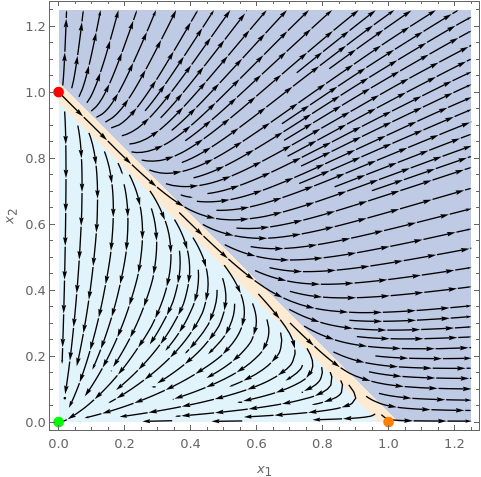
\includegraphics[width=0.6\columnwidth]{figures/dynamical-system.png}
    \caption[Stream plot of the phase space for the dynamical system of a cosmological model with a function $f(Q)$ that replicates dark energy.]
    {Stream plot of the phase space for the dynamical system being studied where the fixed point \textit{I} (stable) is represented in green, fixed point \textit{II} (saddle) in orange and fixed point \textit{III} (unstable) is in red. The light blue marks the region where $\lambda > 0$, the light brown region corresponds to $\lambda = 0$ and the dark blue region to $\lambda < 0$.}
    \label{fig:dynamical-system}
\end{figure}

We can see that for any initial state of the universe which falls inside region \textit{A}, it follows that the final state of the universe will always be fixed point \textit{I}, which corresponds to a eternal inflation.

However, if the initial state of the universe happens to be in the line corresponding to region \textit{B}, the universe will repel away from the fixed point \textit{III}, a radiation dominated epoch, and flow towards fixed point \textit{II}, a matter dominated epoch, which will be the ultimate fate of the universe.

As for region \textit{C}, as it was mentioned before, there are no fixed points and all trajectories diverge towards infinity. This means that both $x_1$ and $x_2$ will increase perpetually implying that the scale factor must decrease and asymptotically approach zero, which physically corresponds to a universe with a big crunch.

Current observations of the state of the universe suggest that we are headed towards a scenario of never-ending expansion. From these the three disjoint regions only the first is able to agree with observations. As such, this forces us to assume that $\lambda$ must be positive, which is in agreement to what was obtained in \cite{Anagnostopoulos2021}, where this model was constrained using current observations from different sources of data.

If we insert the function $f(Q)$ we are considering for this model, introduced in \cref{eq:STG-dark-energy-model}, in the modified first Friedmann equation, presented in \cref{eq:STG-friedmann-1}, we can relate the value of $\lambda$ with both $\Omega_m$ and $\Omega_r$ as

\begin{equation}
    \label{eq:STG-dark-energy-friedmann-1}
    (E^2 - 2\lambda)e^{\lambda/E^2} = \Omega_m (1+z)^3 + \Omega_r (1+z)^4 \,,
\end{equation}
which when considered for the present day and performing some rearrangements yields

\begin{equation}
    \label{eq:STG-dark-energy-omegas-conservation}
    \left( \lambda - \frac{1}{2} \right) e^{\lambda - 1/2} = - \frac{\Omega_m + \Omega_r}{2e^{1/2}} \,.
\end{equation}

The previous system only possesses a solution if we require that the sum of the densities to be lower than $2 e^{-1/2}$. This is not immediately ensured because, unlike what happens in \gls{LCDM} where the sum of the densities is always equal to 1, here the first Friedmann equation is modified, setting no boundaries on the sum of the densities today. Taking this upper bound into consideration, and also the fact that each of the densities are always positive, then the right hand side of the previous equation obeys the inequality

\begin{equation}
    -\frac{1}{e} \leq - \frac{\Omega_m + \Omega_r}{2e^{1/2}} < 0 \,,
\end{equation}
and thus we are able to express the possible solutions for $\lambda$ as

\begin{equation}
    \lambda_0 = \frac{1}{2} + W_0\left( -\frac{\Omega_m + \Omega_r}{2e^{1/2}} \right)
    \,, \hspace{1cm}
    \lambda_{-1} = \frac{1}{2} + W_{-1}\left( -\frac{\Omega_m + \Omega_r}{2e^{1/2}} \right)
    \,,
\end{equation}
where $W_0$ and $W_{-1}$ are the main and the $-1$ branch of the Lambert function respectively.

We can see that there are two possible solutions for the value of $\lambda$. However, as we have previously discussed, the value of $\lambda$ must be positive in order for the model to agree with observations. Looking at both branches, we can see that the value of $\lambda_{-1}$ is strictly negative, leaving $\lambda_0$ as the only physically meaningful solution to this problem. Additionally, we see that the value of $\lambda_0$ takes negative values when $\Omega_m + \Omega_r > 1$. This means that, in order to agree with observations at all times, the sum of the densities must satisfy the constraint $\Omega_m + \Omega_r < 1$, which is familiar to us given that this is what one expects from \gls{LCDM}.


%---------------------------------------------------------------------------------------------------
% Model Selection using Standard Sirens
%---------------------------------------------------------------------------------------------------
\section{Model Selection using Standard Sirens}
\label{sec:fQ-dark-energy-forecasts}

In this section we will be using \gls{SS} mock catalogs to see whether future data will be able to distinguish this model from \gls{LCDM} apart. It is important to note that, just like in the previous model, we neglect the effect of radiation from now on, on the basis that \gls{SS} are not expected to take place in epochs where radiation plays an important role.

Inserting the function $f(Q)$ specific for this model, given in \cref{eq:STG-dark-energy-model}, in the generic form for the luminosity distance of \glspl{GW} for a cosmological model based on $f(Q)$ gravity, presented in \cref{eq:STG-generic-dLGW}, we obtain

\begin{equation}
    d_L^\text{(GW)}(z) = \sqrt{ \frac{1 - \lambda}{1 - \lambda/E^2}} e^{\frac{\lambda}{2}(1 - 1/E^2)} d_L(z) \,.
\end{equation}

Using the model selection criteria introduced in \cref{sec:model-selection-criteria}, we take the best \gls{LISA} catalog, as well as the single \gls{ET} catalog, and compute the corresponding values of the \gls{elpd} using \gls{PSIS-LOO-CV} for this model and \gls{LCDM}. The results for the model selection criteria are presented in \cref{tab:elpd-SS}, whereas the best-fit values are shown in \cref{tab:fotis-best-fit}. Additionally, the best-fit for the model presented in \cref{eq:STG-dark-energy-model} and $\Lambda$CDM when using data from the \gls{ET} are presented in \cref{fig:SS-fotisvsLCDM.png}.

\vspace{0.5cm}

\begin{table}[h!]
    \centering
    \begin{tabular}{|c|cc|}
        \hline
        \multirow{2}{*}{Model} & \multicolumn{2}{c|}{elpd}                                     \\ \cline{2-3}
                               & \multicolumn{1}{c|}{LISA (best)}       & ET                   \\ \hline
        $f(Q)$ as Dark Energy  & \multicolumn{1}{c|}{$-19.58 \pm 7.17$} & $-1720.99 \pm 36.50$ \\ \hline
        $\Lambda$CDM           & \multicolumn{1}{c|}{$-19.76 \pm 7.19$} & $-1721.00 \pm 36.52$ \\ \hline
    \end{tabular}
    \caption
    [The average of the elpd, computed using PSIS-LOO-CV, for a model of $f(Q)$ as Dark Energy and $\Lambda$CDM, for the best LISA catalog and the single ET catalog.]
    {The average of the \gls{elpd}, computed using \gls{PSIS-LOO-CV}, for the model given by \cref{eq:STG-dark-energy-model} and $\Lambda$CDM, for the best \gls{LISA} catalog and the single \gls{ET} catalog.}
    \label{tab:elpd-SS}
\end{table}

\begin{figure}[h!]
    \centering
    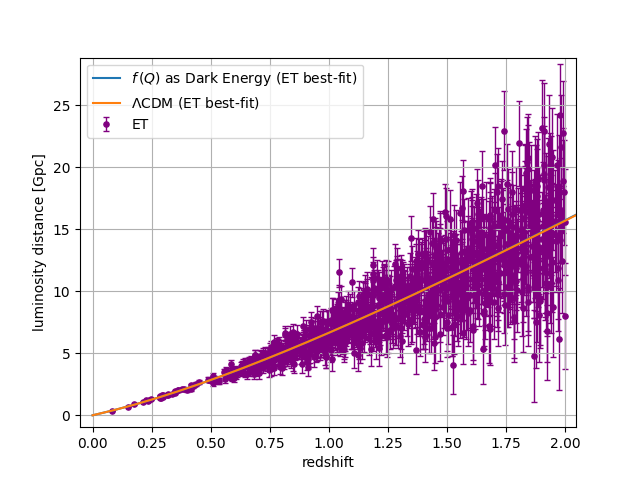
\includegraphics[width=0.67\columnwidth]{figures/SS-fotisvsLCDM.png}
    \caption
    [The best-fit luminosity distance curve, in Gpc, versus the redshift for a model of $f(Q)$ as dark energy and $\Lambda$CDM, when using data from the ET.]
    {The best-fit luminosity distance curve, in Gpc, versus the redshift for model \cref{eq:STG-dark-energy-model} and $\Lambda$CDM, when using data from the \gls{ET}.}
    \label{fig:SS-fotisvsLCDM.png}
\end{figure}

\begin{table}[h!]
    \centering
    \begin{tabular}{|c|cc|cc|}
        \hline
        \multirow{2}{*}{Model} & \multicolumn{2}{c|}{$h$}              & \multicolumn{2}{c|}{$\Omega_m$}       \\ \cline{2-5}
                               & \multicolumn{1}{c|}{LISA (best)} & ET & \multicolumn{1}{c|}{LISA (best)} & ET \\ \hline
        $f(Q)$ as Dark Energy & \multicolumn{1}{c|}{$0.7118 \pm 0.0092$} & $0.6989 \pm 0.0057$ & \multicolumn{1}{c|}{$0.205^{+0.021}_{-0.025}$} & $0.257 \pm 0.016$ \\ \hline
        $\Lambda$CDM          & \multicolumn{1}{c|}{$0.7127 \pm 0.0093$} & $0.6995 \pm 0.0058$ & \multicolumn{1}{c|}{$0.236^{+0.023}_{-0.026}$} & $0.290 \pm 0.017$ \\ \hline
    \end{tabular}
    \caption
    [The best fit values and corresponding 1$\sigma$ region for both $h$ and $\Omega_m$, for a model of $f(Q)$ as Dark Energy and $\Lambda$CDM, for the best LISA catalog and the single ET catalog.]
    {The best fit values and corresponding 1$\sigma$ region for both $h$ and $\Omega_m$, for the model given by \cref{eq:STG-dark-energy-model} and \gls{LCDM}, for the best \gls{LISA} catalog and the single \gls{ET} catalog.}
    \label{tab:fotis-best-fit}
\end{table}

Based on the results presented in \cref{tab:elpd-SS} we can conclude that the two models behave similarly when it comes to predicting held-out data. Looking at \cref{fig:SS-fotisvsLCDM.png} we can see that there is an overlap between the best-fits of the luminosity distance of both models, and that both replicate the original distribution used to create the \gls{SS} events, meaning that both fit the data well. This goes to show that this model is essentially indistinguishable from \gls{LCDM}.

The lower values of the \gls{elpd} for the \gls{ET} when compared to \gls{LISA} are explained due to the higher number of events the former has when compared to the later, as discussed in \cref{sec:model-selection-criteria}.

From \cref{tab:fotis-best-fit} it is possible to see that, for a given catalog, the best fit values of $\Omega_m$ for both \gls{LCDM} and for the model we are considering, agree on the value of $h$, but do not agree on the value of $\Omega_m$. It is important to note that the value of $\Omega_m$ obtained for \gls{LISA} and for the \gls{ET} are lower than expected. However, this was merely a statistical fluctuations, as when consider the other \gls{LISA} catalogs there are others which feature a larger value of $\Omega_m$.

All other mock catalogs which we have applied model selection criteria to revealed, with different degrees of precision, results that agree with the conclusions that we have just discussed. This is something we expected, since if we are unable to distinguish between two models with the best catalogs, then it is not expected that any of the other catalogs are able to differentiate between the two.

We would also like to note that the constraining power of a given catalog for the previous model is the almost the same as when considering this catalog, meaning that a good (or bad) catalog for the previous model is also a good (or bad) catalog for this model.


%-------------------------------------------------
\subsection{Varying the Number of Events}
\label{subsec:variable-number}
%-------------------------------------------------

Given that we are unable to distinguish between the two models with the mock catalogs we have generated, we then asked ourselves whether this was a matter of precision, and decided to investigate whether it is possible to increase the number of \gls{SS} events such that differences between this model and \gls{LCDM} could be observed.

In order to minimize statistical fluctuations, for each number of events per catalog, represented by $N$, we generate $J$ different catalogs. Each catalog, which we index by the letter $j$ ranging from $j = 1$ to $j = J$, will then be used to compute the value of \gls{elpd} using \gls{PSIS-LOO-CV}. The final result is provided by averaging out the values obtained for all catalogs with the same $N$, propagating the uncertainties according to the standard rules of propagation of uncertainty.

For \gls{LISA} we take $N = 5, 10, 15, 20, 25, 30$ events per catalog, and generate $J = 15$ different catalogs. For the \gls{ET} we take $N = 500, 750, 1000, 1250, 1500, 1750$, and generate $J = 5$ catalogs. As for \gls{LIGO}-Virgo, no realistic number of events were able to set constrains on this model.

The absolute value of the average of the \gls{elpd}, computed by \gls{PSIS-LOO-CV} as well as the corresponding error, as a function of the number of events per catalog $N$ obtained for \gls{LISA} is represented in the left plot of \cref{fig:elpd}, whereas the results obtained for the \gls{ET} are present on the right plot.

\begin{figure}[h!]
    \centering
    \begin{subfigure}[b]{0.495\textwidth}
        \centering
        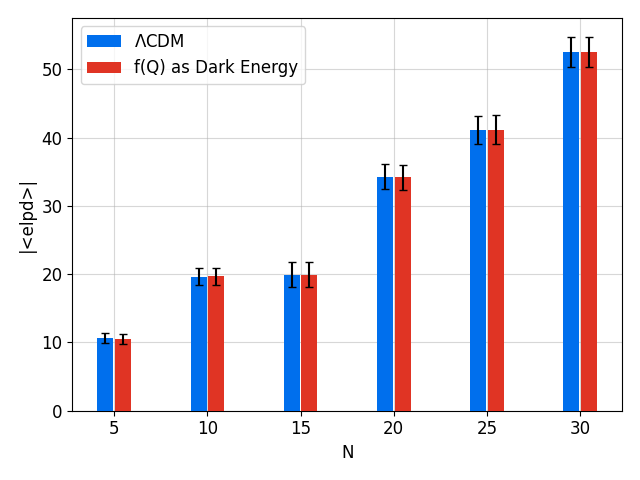
\includegraphics[width=\textwidth]{figures/elpd-LISA.png}
    \end{subfigure}
    \hfill
    \begin{subfigure}[b]{0.495\textwidth}
        \centering
        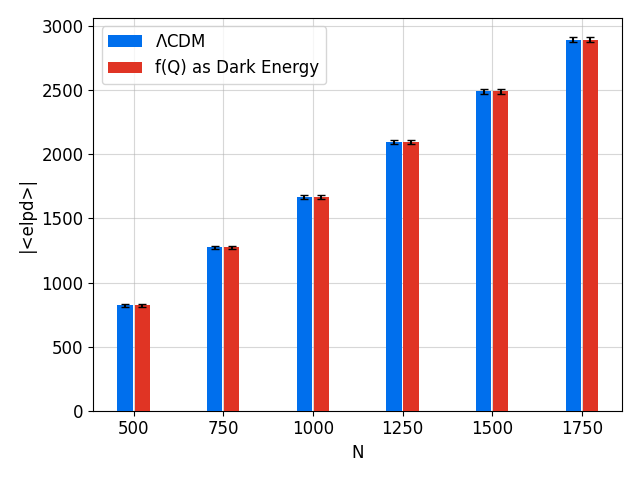
\includegraphics[width=\textwidth]{figures/elpd-ET.png}
    \end{subfigure}
    \caption[The absolute value of the average of the elpd, computed by PSIS-LOO-CV, for a model of $f(Q)$ as dark energy and $\Lambda$CDM, when considering all catalogs with the same number of events per catalog. The plot on the left was made using data coming from LISA, whereas the one on the right uses data coming from the ET.]
    {The absolute value of the \gls{elpd}, computed by \gls{PSIS-LOO-CV}, for both the model presented in \cref{eq:STG-dark-energy-model} and \gls{LCDM}, when considering all catalogs with the same number of events per catalog. The plot on the left was made using data coming from \gls{LISA}, whereas the one on the right uses data coming from the \gls{ET}.}
    \label{fig:elpd}
\end{figure}

\begin{figure}[h!]
    \centering
    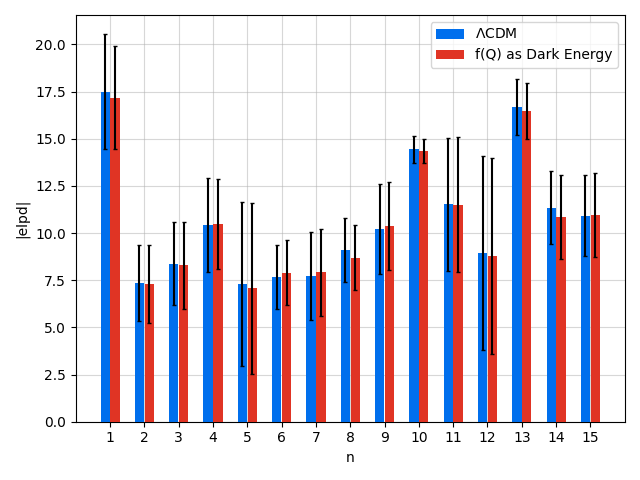
\includegraphics[width=0.7\columnwidth]{figures/elpd-LISA-N15.png}
    \caption
    [The absolute value of the elpd, computed by PSIS-LOO-CV, for both a model of $f(Q)$ as Dark Energy and $\Lambda$CDM, for all LISA catalogs with 15 events per catalog.]
    {The absolute value of the \gls{elpd}, computed by \gls{PSIS-LOO-CV}, for both the model presented in \cref{eq:STG-dark-energy-model} and \gls{LCDM}, for all \gls{LISA} catalogs with $N = 15$ events per catalog.}
    \label{fig:elpd-LISA-N15}
\end{figure}

The most important observation we can make is that, regardless of the value of $N$, and whether we are considering \gls{LISA} or the \gls{ET}, the value of the \gls{elpd} tells us that these two models behave equally well on predicting held-out data. In fact, this equivalence is stronger, since this is something which happens on a per catalog basis. As an example we show in \cref{fig:elpd-LISA-N15} the value of the \gls{elpd} for all \gls{LISA} catalogs with $N = 15$.

We can therefore extrapolate that, regardless of the number of \gls{SS} events that we are to consider, the luminosity distance curve for this model is able to closely match the luminosity distance curve for \gls{LCDM}.

It is important to note that all values of the \gls{elpd} are negative, as we have remarked in \cref{sec:model-selection-criteria}. The absolute value is shown instead to increase the readability of the figures. The decreasing value of the \gls{elpd} with increasing $N$ is explained using the same reasoning presented in \cref{sec:model-selection-criteria}, which is that more events will always decrease the value of the \gls{elpd}.


%-------------------------------------------------
% Using Type Ia Supernovae
%-------------------------------------------------
\subsection{Using Type Ia Supernovae}
\label{subsec:data-from-SNIa}

The exercise in the previous section clearly shows that it is not possible to distinguish this model from \gls{LCDM} based on \gls{SS} alone, regardless of how many we expect to observe. We will now add current \gls{SNIa} data and again apply model selection criteria to see whether this dataset prefers the model given by \cref{eq:STG-dark-energy-model} or $\Lambda$CDM. Because of the marginalization's performed on the likelihood for \gls{SNIa}, in order to remove the degeneracy between $M$ and $H_0$, we are only able to constrain the value of $\Omega_m$ using this dataset.

Applying the model selection criteria, we present the values of the \gls{elpd} computed using \gls{PSIS-LOO-CV} in \cref{tab:elpd-SNIa}. In \cref{fig:SNIa-fotisvsLCDM.png} we present the best-fit curves of the logarithm of the $H_0$ independent luminosity distance function as a function of redshift, $5 \log {D_L(z)}$, as well as the events from the Pantheon sample.

\begin{figure}[h!]
    \centering
    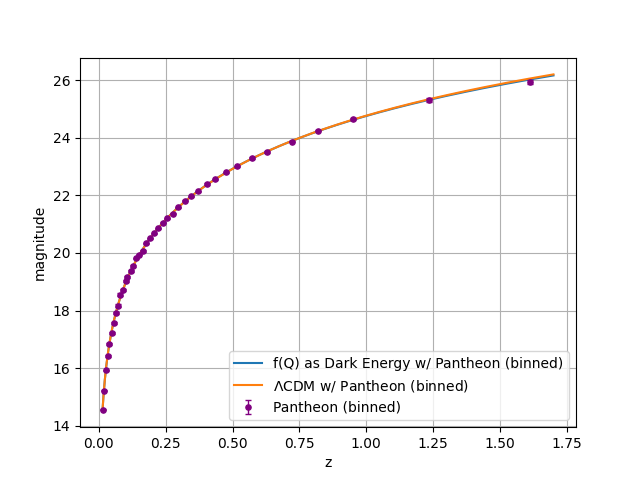
\includegraphics[width=0.7\columnwidth]{figures/SNIa-fotisvsLCDM.png}
    \caption
    [The best fit of the logarithm of the $H_0$ independent luminosity distance, $5 \log{D_L(z)}$, versus redshift for a model of $f(Q)$ as dark energy and $\Lambda$CDM, as well as the magnitude versus redshift of the Pantheon events.]
    {The best fit of the logarithm of the $H_0$ independent luminosity distance, $5 \log{D_L(z)}$, versus redshift for the model in \cref{eq:STG-dark-energy-model} and \gls{LCDM}, as well as the magnitude versus redshift of the Pantheon events.}
    \label{fig:SNIa-fotisvsLCDM.png}
\end{figure}

\begin{table}[h!]
    \centering
    \begin{tabular}{|c|c|}
        \hline
        Model                & elpd              \\ \hline
        $f(Q$ as Dark Energy & $-24.47 \pm 6.21$ \\ \hline
        $\Lambda$CDM         & $-25.83 \pm 6.22$ \\ \hline
    \end{tabular}
    \caption
    [The value of the elpd, computed by PSIS-LOO-CV, for a model of $f(Q)$ as Dark Energy and $\Lambda$CDM, when considering SNIa from the Pantheon sample.]
    {The value of the \gls{elpd}, computed by \gls{PSIS-LOO-CV}, for the model presented in \cref{eq:STG-dark-energy-model} and \gls{LCDM}, when considering \gls{SNIa} from the Pantheon sample.}
    \label{tab:elpd-SNIa}
\end{table}

From \cref{fig:SNIa-fotisvsLCDM.png} we can see that the best-fits for each model are essentially indistinguishable, and seem to be in agreement with the observations considered. As measured quantitatively by \cref{tab:elpd-SNIa}, both models behave equally well on predicting held-out data, which means that \gls{SNIa} are unable to distinguish this model from \gls{LCDM}.

From the constraining procedure using \gls{SNIa} from the Pantheon sample, we have obtained the value of $\Omega_m = 0.335 \pm 0.012$ for the model which we are studying in this chapter, and $\Omega_m = 0.285 \pm 0.012$ for \gls{LCDM}.

If we now remember the constrains set on this model using \gls{SS} events, which was already presented in \cref{tab:fotis-best-fit}, we obtained a value for the matter density of $\Omega_m = 0.257 \pm 0.016$ when using the \gls{ET}. Comparing the constrains set by the \gls{SS} and \gls{SNIa}, it is easy to see that there exists a tension between the datasets. In \cref{fig:SNIa-tension} we show the corner plot where we have constrained this model (on the left subplot) and \gls{LCDM} (on the right subplot) with \gls{SS} events from the \gls{ET}, \gls{LISA} (both the median and best catalog) and \gls{SNIa} alone.

\begin{figure}[h!]
    \begin{subfigure}[b]{0.495\textwidth}
        \centering
        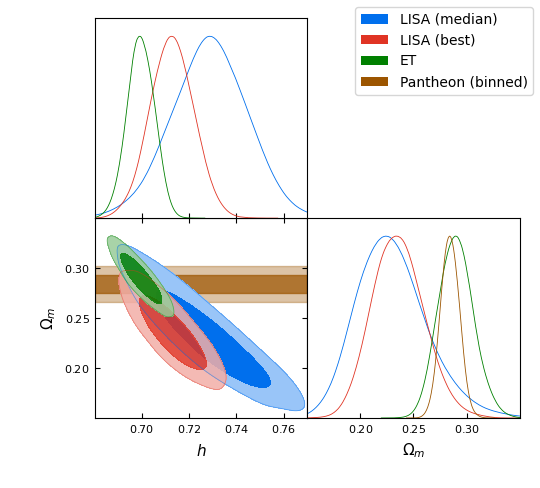
\includegraphics[width=\textwidth]{figures/LCDM-SNIa-tension.png}
    \end{subfigure}
    \hfill
    \centering
    \begin{subfigure}[b]{0.495\textwidth}
        \centering
        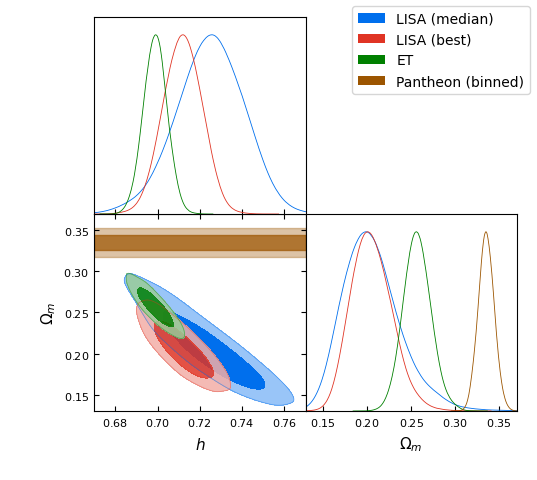
\includegraphics[width=\textwidth]{figures/fotis-SNIa-tension.png}
    \end{subfigure}
    \caption
    [Constrains set by the ET, the best and median LISA catalog and SNIa from the Pantheon sample alone, for $\Lambda$CDM (on the left) and for a model of $f(Q)$ which replicates dark energy (on the right).]
    {Constrains set by the \gls{ET}, the best and median \gls{LISA} catalog as well as \gls{SNIa} from the Pantheon sample alone, for \gls{LCDM} (on the left) and for the model given in \cref{eq:STG-dark-energy-model} (on the right).}
    \label{fig:SNIa-tension}
\end{figure}

From \cref{fig:SNIa-tension} it is easy to see that although the events coming from \gls{SS} are in very good agreement with the data from \gls{SNIa} in \gls{LCDM}, the same does not hold true for this model. As such, we can conclude that if \gls{LCDM} with values of $h = 0.7$ and $\Omega_m = 0.284$ is the model which accurately describes the evolution of the universe, then it is expected that future \gls{SS} events, along with current \gls{SNIa} data, will be able to rule this model of $f(Q)$ gravity out. Until then, this model might very well be indistinguishable from \gls{LCDM} due to its close similarity with it.

To provide a more quantitative view of the existing tension, in \cref{tab:SNIa-tensions} we present the number of sigmas between the best-fit of $\Omega_m$ for that catalog and the value of $\Omega_m$ given by the Pantheon sample. This table does not include the worst \gls{LISA} catalog, due to its remarkably low constraining power when compared to all of the other catalogs.

\begin{table}[h!]
    \centering
    \begin{tabular}{|c|c|}
        \hline
        Dataset                            & $\sigma$'s to Pantheon $\Omega_m$ best-fit \\ \hline
        ET                                 & 4.9                                        \\ \hline
        LISA (best)                        & 5.7                                        \\ \hline
        LISA (median)                      & 4.2                                        \\ \hline
        LISA (worst) + LIGO-Virgo (best)   & 4.6                                        \\ \hline
        LISA (worst) + LIGO-Virgo (median) & 2.0                                        \\ \hline
        LISA (worst) + LIGO-Virgo (worst)  & 3.2                                        \\ \hline
    \end{tabular}
    \caption
    [The number of sigmas between the best-fit value for $\Omega_m$ for each dataset and the Pantheon best-fit, for a model of $f(Q)$ which replicates dark energy. The value of $\sigma_{\Omega_m}$ used is referent to each dataset.]
    {The number of sigmas between the best-fit value for $\Omega_m$ between each catalog and the Pantheon best-fit, for the model presented in \cref{eq:STG-dark-energy-model}. The value of $\sigma$ being considered is referent to each dataset.}
    \label{tab:SNIa-tensions}
\end{table}


%---------------------------------------------------------------------------------------------------
\section{Summary}
\label{sec:STG-dark-energy-summary}
%---------------------------------------------------------------------------------------------------

In this chapter, we studied an $f(Q)$ model which aims to replace dark energy with a modification of gravity, and introduces no additional free parameters, since the parameter $\lambda$ which was added on the action can be expressed as a function of the densities. This model approaches \gls{GR} as the redshift increase, meaning that deviations from \gls{LCDM} only happen in the low redshift regime.

This model was then studied using dynamical system analysis, which reveals three fixed points, of which only one of them is stable, and represents a scenario of permanent inflation. The system is separated into three disjoint regions, which are categorized by the sign of $\lambda$. The region with $\lambda > 0$ is the one that includes the stable fixed point, and the evolution of the universe will therefore always go towards permanent inflation. For the case where $\lambda = 0$, we fall back to \gls{STEGR}, but not to \gls{LCDM}, due to the lack of dark energy, meaning that we have a \gls{CDM} universe. In this region, all trajectories flow from a radiation dominated epoch to a matter dominated epoch. The final region, which features $\lambda > 0$, has no fixed points and all trajectories point towards a big crunch.

We used model selection criteria using \gls{SS} to attempt to distinguish this model from \gls{LCDM} apart, only to conclude that no number of \gls{SS} events is expected to be able to do so. We then decided to increase the number of \gls{SS} events in each dataset, and see whether applying model selection criteria would allow us to tell this model from \gls{LCDM} apart. This analysis showed that we do not expect to be able to tell between these two model apart by increasing the number of \gls{SS} events we expect to measure. Due to the fact that the best-fit for the luminosity distance curves for both models are indistinguishable, we believe that no number of \gls{SS} events will be able to prefer one model over the other.

Using \gls{SNIa} data from the Pantheon sample, we showed that both models provide similar best-fits and are equially good at predicting held-out data. However, by constraining this model using \gls{SNIa} we had a best-fit of $\Omega_m = 0.3353 \pm 0.0091$, whereas when using \gls{SS} events from the \gls{ET} we obtained a value of $\Omega_m = 0.257 \pm 0.016$, implying that there is a tension in this model when considering different sources of data. This means that, if our fiducial cosmology is in fact true, then \gls{SS} are expected to give rise to a tension in this model, and effectively rule it out.
